% M1-v0: strcpy vào order_id[16] (CÓ LỖI)
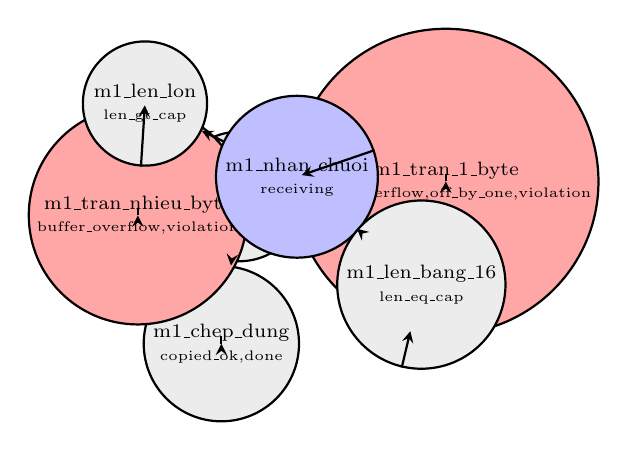
\begin{tikzpicture}[
  every node/.style={draw, circle, inner sep=2pt,
      minimum size=8mm, align=center, font=\scriptsize},
  ->, >=stealth, thick, auto
]
  \node[fill=gray!15] (nd_m1_len_nho) at (-0.42,0.23) {m1\_len\_nho\\{\tiny len\_lt\_cap}};
  \node[fill=red!35] (nd_m1_tran_1_byte) at (2.20,0.42) {m1\_tran\_1\_byte\\{\tiny buffer\_overflow,off\_by\_one,violation}};
  \node[fill=gray!15] (nd_m1_chep_dung) at (-0.65,-1.64) {m1\_chep\_dung\\{\tiny copied\_ok,done}};
  \node[fill=red!35] (nd_m1_tran_nhieu_byte) at (-1.71,-0.01) {m1\_tran\_nhieu\_byte\\{\tiny buffer\_overflow,violation}};
  \node[fill=blue!25] (nd_m1_nhan_chuoi) at (0.31,0.48) {m1\_nhan\_chuoi\\{\tiny receiving}};
  \node[fill=gray!15] (nd_m1_len_lon) at (-1.62,1.41) {m1\_len\_lon\\{\tiny len\_gt\_cap}};
  \node[fill=gray!15] (nd_m1_len_bang_16) at (1.89,-0.89) {m1\_len\_bang\_16\\{\tiny len\_eq\_cap}};
  \draw (nd_m1_len_nho) -- (nd_m1_chep_dung);
  \draw (nd_m1_tran_1_byte) -- (nd_m1_tran_1_byte);
  \draw (nd_m1_chep_dung) -- (nd_m1_chep_dung);
  \draw (nd_m1_tran_nhieu_byte) -- (nd_m1_tran_nhieu_byte);
  \draw (nd_m1_nhan_chuoi) -- (nd_m1_len_bang_16);
  \draw (nd_m1_nhan_chuoi) -- (nd_m1_len_nho);
  \draw (nd_m1_nhan_chuoi) -- (nd_m1_len_lon);
  \draw (nd_m1_len_lon) -- (nd_m1_tran_nhieu_byte);
  \draw (nd_m1_len_bang_16) -- (nd_m1_tran_1_byte);
\end{tikzpicture}

% M1-v1a: bản 'an toàn' phần mềm sinh — strncpy(buf,src,15) (CẮT CỤT)
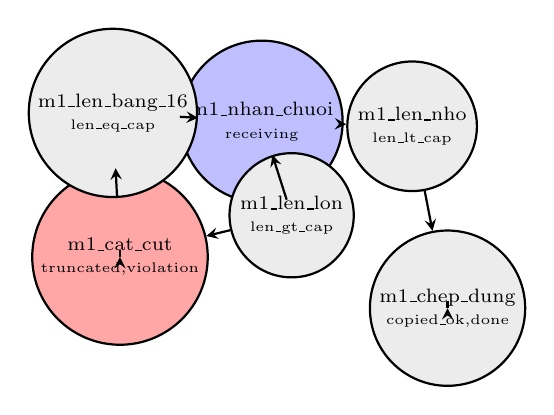
\begin{tikzpicture}[
  every node/.style={draw, circle, inner sep=2pt,
      minimum size=8mm, align=center, font=\scriptsize},
  ->, >=stealth, thick, auto
]
  \node[fill=gray!15] (nd_m1_len_nho) at (1.75,0.81) {m1\_len\_nho\\{\tiny len\_lt\_cap}};
  \node[fill=gray!15] (nd_m1_chep_dung) at (2.20,-1.50) {m1\_chep\_dung\\{\tiny copied\_ok,done}};
  \node[fill=blue!25] (nd_m1_nhan_chuoi) at (-0.16,0.87) {m1\_nhan\_chuoi\\{\tiny receiving}};
  \node[fill=red!35] (nd_m1_cat_cut) at (-1.96,-0.85) {m1\_cat\_cut\\{\tiny truncated,violation}};
  \node[fill=gray!15] (nd_m1_len_lon) at (0.22,-0.32) {m1\_len\_lon\\{\tiny len\_gt\_cap}};
  \node[fill=gray!15] (nd_m1_len_bang_16) at (-2.05,0.98) {m1\_len\_bang\_16\\{\tiny len\_eq\_cap}};
  \draw (nd_m1_len_nho) -- (nd_m1_chep_dung);
  \draw (nd_m1_chep_dung) -- (nd_m1_chep_dung);
  \draw (nd_m1_nhan_chuoi) -- (nd_m1_len_bang_16);
  \draw (nd_m1_nhan_chuoi) -- (nd_m1_len_nho);
  \draw (nd_m1_nhan_chuoi) -- (nd_m1_len_lon);
  \draw (nd_m1_cat_cut) -- (nd_m1_cat_cut);
  \draw (nd_m1_len_lon) -- (nd_m1_cat_cut);
  \draw (nd_m1_len_bang_16) -- (nd_m1_cat_cut);
\end{tikzpicture}

% M1-v1b: bản sửa của nhóm — buf[17] + strnlen + từ chối
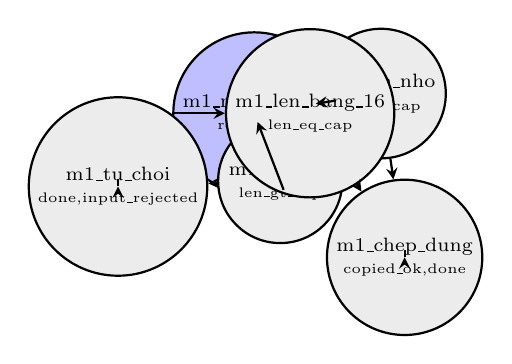
\begin{tikzpicture}[
  every node/.style={draw, circle, inner sep=2pt,
      minimum size=8mm, align=center, font=\scriptsize},
  ->, >=stealth, thick, auto
]
  \node[fill=gray!15] (nd_m1_len_nho) at (1.14,0.81) {m1\_len\_nho\\{\tiny len\_lt\_cap}};
  \node[fill=gray!15] (nd_m1_chep_dung) at (1.44,-1.27) {m1\_chep\_dung\\{\tiny copied\_ok,done}};
  \node[fill=blue!25] (nd_m1_nhan_chuoi) at (-0.47,0.56) {m1\_nhan\_chuoi\\{\tiny receiving}};
  \node[fill=gray!15] (nd_m1_tu_choi) at (-2.20,-0.37) {m1\_tu\_choi\\{\tiny done,input\_rejected}};
  \node[fill=gray!15] (nd_m1_len_lon) at (-0.14,-0.30) {m1\_len\_lon\\{\tiny len\_gt\_cap}};
  \node[fill=gray!15] (nd_m1_len_bang_16) at (0.24,0.56) {m1\_len\_bang\_16\\{\tiny len\_eq\_cap}};
  \draw (nd_m1_len_nho) -- (nd_m1_chep_dung);
  \draw (nd_m1_chep_dung) -- (nd_m1_chep_dung);
  \draw (nd_m1_nhan_chuoi) -- (nd_m1_len_bang_16);
  \draw (nd_m1_nhan_chuoi) -- (nd_m1_len_nho);
  \draw (nd_m1_nhan_chuoi) -- (nd_m1_len_lon);
  \draw (nd_m1_tu_choi) -- (nd_m1_tu_choi);
  \draw (nd_m1_len_lon) -- (nd_m1_tu_choi);
  \draw (nd_m1_len_bang_16) -- (nd_m1_chep_dung);
\end{tikzpicture}